\subsection{Motivación}

\begin{frame}
	\frametitle{Motivación}
	\begin{itemize}
	\item	Muchas aplicaciones de las bases de datos deben tener
		en cuenta la temporalidad de los datos. \pause
		Aplicaciones financieras, compañías de seguro, reserva
		de hoteles, registros de pacientes, sistemas de soporte
		a la decisión. \pause

	\item	Si bien se puede manejar desde un nivel mas alto, esto
		complica las consultas SQL y se vuelve inmanejable rápidamente.
		\pause

	\item	Por eso, queremos tener motores que sean ``conscientes'' de
		la temporalidad, con un lenguaje especializado.
	\end{itemize}
\end{frame}

\begin{frame}
\frametitle{Definición de DB Temporal}
	\begin{itemize}
	\item	Una DB Temporal es una DB con soporte interno para manejar
		datos temporales. \pause

	\item	Existen 3 tipos: \pause
		\begin{itemize}
		\item Histórica: mantiene el tiempo de validez \pause
		\item Rollback: mantiene el tiempo de transacción \pause
		\item Bitemporales: mantiene ambos \pause
		\end{itemize}

	\item	A su vez, pueden implementarse con timestamps por tupla
		o por atributo. Vamos a estudiar las estampadas por tuplas
		en detalle.
	\end{itemize}
\end{frame}

\begin{frame}
\frametitle{Tiempo de transacción y tiempo de validez}
	\begin{itemize}
	\item	El tiempo de {\bf validez} indica cuando una entrada de la DB
		tiene validez en la realidad que se modela. \pause Puede
		ser un intervalo completamente en el pasado, del pasado al
		futuro, o en el futuro enteramente.
	\pause
	\item	El tiempo de {\bf transacción} indica cuando la tupla se añadió
		a la DB cómo válida, y cuando se dejó de creer en su validez.
		\pause Esto permite saber que es lo que la DB ``creía'' en
		un momento determinado del pasado.
		\pause Nunca puede haber un tiempo futuro.
	\end{itemize}
\end{frame}

\begin{frame}
\frametitle{Tiempo de transacción y tiempo de validez}
	\begin{itemize}
	\item	Los tiempos de validez y de transacción están en dos escalas
		completamente distintas. \pause
		Si estamos modelando eventos del siglo 18, los tiempos de validez
		irán del 1700 al 1799. \pause
		Sin embargo, los de transacción irán de la fecha de creación
		de la DB hasta el presente.
	\end{itemize}
\end{frame}

\begin{frame}
	\begin{center}
	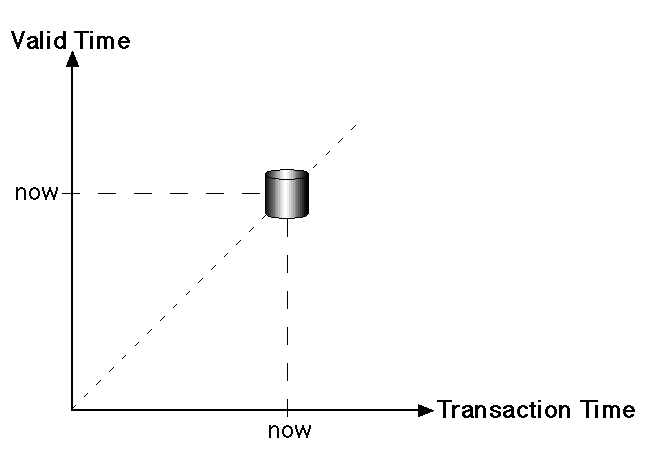
\includegraphics[height=5cm]{snapshot.png}
	\end{center}
\end{frame}

\begin{frame}
	\begin{center}
	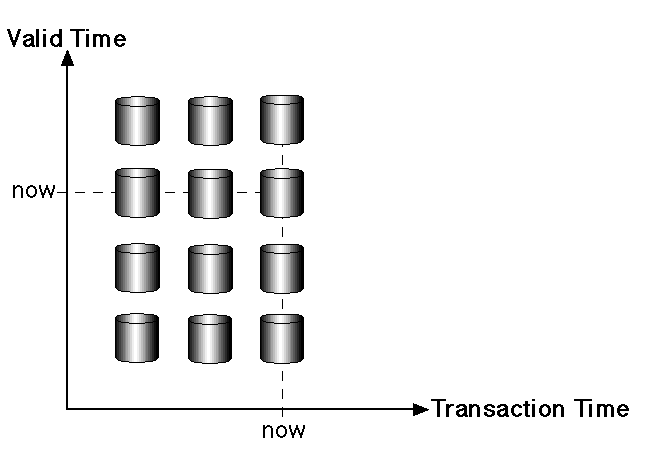
\includegraphics[height=5cm]{bitemporal.png}
	\end{center}
\end{frame}

\begin{frame}
\begin{center}
\frametitle{Ejemplo de bitemporalidad}
	\tiny

	``Desde el 1/6/1995 al 3/9/2000 John se mudó a Beachy, pero para no
	pagar impuestos, nuncá lo reportó. Luego, durante una investigación
	se descubre (en el 2/2/2001) que si se había mudado.''

	\pause
	\vspace{5mm}

	Histórica: \hfill
	\begin{tabular}{|c|c|c|c|}
	\hline
	Nombre   & Ciudad	& ValidFrom	& ValidTo	\\ \hline
	John Doe & Smallville	& 3/4/1975	& 26/8/1994	\\ \hline
	John Doe & Bigtown	& 26/8/1994	& 1/6/1995	\\ \hline
	John Doe & Beachy	& 1/6/1995	& 3/9/2000	\\ \hline
	John Doe & Bigtown	& 3/9/2000	& 1/4/2001	\\ \hline
	\end{tabular}

	\pause
	\vspace{5mm}

	\newcommand{\z}[0]{\alert<4>}

	Bitemporal: \hfill
	\begin{tabular}{|c|c|c|c|c|c|}
	\hline
	Nombre   & Ciudad	& ValidFrom	& ValidTo	& TransFrom	& TransTo	\\ \hline
	John Doe & Smallville	& 3/4/1975	& ∞		& 4/4/1975	& 27/12/1994	\\ \hline
	\z{John Doe} & \z{Smallville}	& \z{3/4/1975}	& \z{26/8/1994}	& \z{27/12/1994}	& \z{∞}	\\ \hline
	John Doe & Bigtown	& 26/8/1994	& ∞		& 27/12/1994	& 2/2/2001	\\ \hline
	\z{John Doe} & \z{Bigtown}	& \z{26/8/1994}	& \z{1/6/1995}	& \z{2/2/2001}	& \z{∞}	\\ \hline
	\z{John Doe} & \z{Beachy}	& \z{1/6/1995}	& \z{3/9/2000}	& \z{2/2/2001}	& \z{∞}	\\ \hline
	John Doe & Bigtown	& 3/9/2000	& ∞		& 2/2/2001	& 1/4/2001	\\ \hline
	\z{John Doe} & \z{Bigtown}	& \z{3/9/2000}	& \z{1/4/2001}	& \z{1/4/2001}	& \z{∞}	\\ \hline
	\end{tabular}
\end{center}
\end{frame}

\begin{frame}
\frametitle{Comparación de tipos de DB Temporal}
	\begin{figure}

	\psmatrix[mnode=r,colsep=1,rowsep=1]
	& [name=1] Bitemporal & \\
	[name=2] Histórica & & [name=3] Rollback \\
	& [name=4] Snapshot &
	\endpsmatrix
	\ncline{<-}{1}{2}
	\ncline{<-}{1}{3}
	\ncline{<-}{2}{4}
	\ncline{<-}{3}{4}
	\end{figure}
\end{frame}

\begin{frame}
\frametitle{Lenguaje temporales}
	\begin{itemize}
	\item	En 1994 se publicó la especificación de TSQL2 como candidato
		para ser el estándar de bases de datos temporales. \pause

	\item	Sin embargo, tuvo críticas por no ser estrictamente relacional
		(\small{\url{http://www.dcs.warwick.ac.uk/~hugh/TTM/OnTSQL2.pdf}}).
		\pause

	\item	El lenguaje SQL-2011 incorpora primitivas para manejar datos temporales.
	\end{itemize}
\end{frame}

\begin{frame}
\frametitle{SQL-2011}
	\begin{itemize}
	\item	No introduce un nuevo tipo para los períodos de tiempo, dado que
		cada usuario del DMBS tendría que adaptarse a los nuevos tipos.
		Esto puede llevar mucho tiempo y hacer que la adoptación del lenguaje
		se atrase. \pause

	\item	Las tablas se crean indicando que ``temporalidad'' queremos. Para el
		tiempo de transacción esto se maneja automáticamente.
		\pause

	\item	Al día de la fecha, no está soportado en MySQL.
	\end{itemize}
\end{frame}

\begin{frame}
\frametitle{SQL-2011 - Creación de tabla histórica}
\begin{center}
\small
	\begin{itemize}

	\item	\texttt{CREATE TABLE Emp(ENo INTEGER, EStart DATE, EEnd DATE,
		EDept INTEGER, PERIOD FOR EPeriod (EStart, EEnd))} \\
	\pause

	\item	\texttt{INSERT INTO Emp VALUES (22217, DATE ‘2010-01-01’,
		DATE '2011-11-12', 3)} \\

	\pause

	\item \begin{tabular}{|c|c|c|c|}
	\hline
	Eno	& EStart	& EEnd		& EDept	\\ \hline
	22217	& 2010-01-01	& 2011-11-12	& 3	\\ \hline
	\end{tabular}

	\pause

	\item	(Nada nuevo hasta ahora)
	\end{itemize}
\end{center}
\end{frame}

\begin{frame}
\frametitle{SQL-2011 - Consultas sobre tabla histórica}
\begin{center}
\small
	\begin{itemize}

	\item	\texttt{UPDATE Emp FOR PORTION OF EPeriod FROM DATE '2011-02-03'
		TO DATE '2011-09-10' SET EDept = 4 WHERE ENo = 22217}
	\pause

	\item Pasamos de: \hfill \begin{tabular}{|c|c|c|c|}
	\hline
	Eno	& EStart	& EEnd		& EDept	\\ \hline
	22217	& 2010-01-01	& 2011-11-12	& 3	\\ \hline
	\end{tabular}
	\pause

	\item A: \hfill \begin{tabular}{|c|c|c|c|}
	\hline
	Eno	& EStart	& EEnd		& EDept	\\ \hline
	22217	& 2010-01-01	& 2011-02-03	& 3	\\ \hline
	22217	& 2011-02-03	& 2011-09-10	& 4	\\ \hline
	22217	& 2011-09-10	& 2011-11-12	& 3	\\ \hline
	\end{tabular}

	\end{itemize}
\end{center}
\end{frame}

\begin{frame}
\frametitle{SQL-2011 - Consultas sobre tabla histórica}
\begin{center}
\small
	\begin{itemize}

	\item	\texttt{DELETE Emp FOR PORTION OF EPeriod FROM DATE '2011-02-03'
		TO DATE '2011-09-10' WHERE ENo = 22217}

	\item Pasamos de: \hfill \begin{tabular}{|c|c|c|c|}
	\hline
	Eno	& EStart	& EEnd		& EDept	\\ \hline
	22217	& 2010-01-01	& 2011-11-12	& 3	\\ \hline
	\end{tabular}

	\item A: \hfill \begin{tabular}{|c|c|c|c|}
	\hline
	Eno	& EStart	& EEnd		& EDept	\\ \hline
	22217	& 2010-01-01	& 2011-02-03	& 3	\\ \hline
	22217	& 2011-09-10	& 2011-11-12	& 3	\\ \hline
	\end{tabular}

	\end{itemize}
\end{center}
\end{frame}

\begin{frame}
\frametitle{SQL-2011 - Clave primaria}
	\begin{itemize}
	\item	En el ejemplo anterior, la clave no puede ser simplemente
		{\it Eno}. \pause

	\item	Agregar los campos del período a la clave tampoco soluciona
		el problema. \pause

		\hfill \begin{tabular}{|c|c|c|c|}
		\hline
		Eno	& EStart	& EEnd		& EDept	\\ \hline
		22217	& 2010-01-01	& 2011-09-10	& 3	\\ \hline
		22217	& 2011-02-03	& 2011-11-12	& 4	\\ \hline
		\end{tabular}
		\pause

	\item	El DBMS nos da soporte interno.
	\pause

	\item	\texttt{ALTER TABLE Emp ADD PRIMARY KEY (ENo, EPeriod WITHOUT OVERLAPS)}
	\end{itemize}
\end{frame}

\begin{frame}
\frametitle{SQL-2011 - Claves foráneas}
	\begin{itemize}
	\item	Se pueden especificar claves foráneas temporales.
		\pause

	\item	El problema:
		\hfill \begin{tabular}{|c|c|c|c|}
		\hline
		Eno	& EStart	& EEnd		& EDept	\\ \hline
		22218	& 2010-01-01	& 2011-02-03	& 3	\\ \hline
		22218	& 2011-02-03	& 2011-11-12	& 4	\\ \hline
		\end{tabular}

		\hfill \begin{tabular}{|c|c|c|c|}
		\hline
		Dno	& DStart	& DEnd		& DName	\\ \hline
		3	& 2009-01-01	& 2011-12-31	& Test	\\ \hline
		4	& 2011-06-01	& 2011-12-31	& QA	\\ \hline
		\end{tabular}
		\pause

	\item	La solución: \texttt{ALTER TABLE Emp ADD FOREIGN KEY (Edept,
			PERIOD EPeriod) REFERENCES Dept (DNo, PERIOD DPeriod)}
	\end{itemize}
\end{frame}

\begin{frame}
\frametitle{SQL-2011 - Condiciones temporales}
	\begin{itemize}
	\item	Para consultar, se puede usar la forma tradicional:

		\texttt{SELECT Name, Edept FROM Emp WHERE ENo = 22217
		AND EStart <= DATE '2011-01-02' AND EEnd > DATE '2011-01-02'}
	\pause

	\item	Sin embargo, hay nuevos operadores que ayudan un poco:

		\texttt{SELECT Ename, Edept FROM Emp WHERE ENo = 22217
		AND EPeriod CONTAINS DATE '2011-01-02'}
	\pause

	\item	Hay mas, como: \texttt{OVERLAPS}, \texttt{EQUALS}, \texttt{PRECEDES},
		\texttt{SUCCEEDS}, \texttt{IMMEDIATELY PRECEDES},
		y \texttt{IMMEDIATELY SUCCEEDS}.
	\end{itemize}
\end{frame}

\begin{frame}
\frametitle{SQL-2011 - Tablas Rollback}
	\begin{itemize}
	\item	Se agregar un período para que el DMBS maneje automáticamente
		con el tiempo de transacción.
	\pause

	\item	\texttt{CREATE TABLE Emp (ENo INTEGER, Sys\_start
		TIMESTAMP(12) GENERATED ALWAYS AS ROW START,
		Sys\_end TIMESTAMP(12) GENERATED ALWAYS AS ROW
		END, EName VARCHAR(30), PERIOD FOR SYSTEM\_TIME
		(Sys\_start, Sys\_end)) WITH SYSTEM VERSIONING}
	\pause

	\item	Al hacer un \texttt{INSERT}, los campos se populan automáticamente
		(Sys\_end vale ∞).
	\pause

	\item	Al hacer \texttt{UPDATE} o \texttt{DELETE} los campos viejos
		son completamente ignorados. Un usuario no puede nunca borrar
		la historia.
	\pause

	\item	No hay implicaciones para claves foráneas.
	\pause

	\item	Se puede hacer un \texttt{SELECT} ``histórico'' con la directiva
		\texttt{FOR SYSTEM\_TIME AS OF}.

	\end{itemize}
\end{frame}
